\chapter{Background}
This chapter provides background information on \textit{location privacy}, and it presents \textit{Enigma}, a theoretical peer-to-peer network that can run computations on multi-sourced data in a privacy preserving manner. It concludes with a discussion over related work, covering the deficiencies of the existing user data markets.

\section{Location Privacy}
\subsection{Location Data}
\textit{Location Data} is a set of data that represents an individual's positions in space over some time period. The granularity of the collected information might vary, depending on the case. 

In the smartphone era, location data is increasingly precise, being emitted in large quantities, due to the technological advancements of the smartphones. However, numerous parties are collecting this data, as part of the agreement of their service provision. Phone carriers usually record this data, and, lately, data location collection is made through the operating system of the phone. The latter makes the information available to any phone application (e.g., Facebook, Google Maps, Snapchat, etc.), as long as the applications have previously obtained the users' agreement.

There have been numerous case studies showing that location data is private sensitive information, and it can be reverse-engineered to uniquely identify its corresponding individual. In one of the most recent papers on the subject, it is claimed that with enough location data collected over a large period (15 months in the study), individuals might be uniquely identified in a crowd of 1.5M people, with an accuracy of 95\%. \cite{datalocation}.

From here, we naturally derive the question of whether it is possible to make data location available to some extent while completely decoupling it from its producer.

\subsection{Overview of Location Privacy}
Generally speaking, location privacy refers to the ability of an individual to move in the spatial dimension, without having their coordinates recorded for a later use.

Since this is a current issue in our present times, various solutions have been proposed, referred to as Location-Privacy Protection Mechanisms (LPPMs) \cite{quantifylocationprivacy}. Each of the proposed LPPMs achieves its ultimate goal to some extent, either by making some initial assumptions about the data providers, or by restricting the types of functions that can be applied over the collected data. Thus, Popa \& co. \cite{privstats} identify two types of location privacy:

\begin{enumerate}
\item \textbf{strict location privacy} - In a system that achieves strict location privacy, the server is not trusted; thus, it can only learn an aggregated result over the location data set.
\item \textbf{differential location privacy} - In a system that achieves differential location privacy, the server is trusted and can have access to the raw set of location data, and their corresponding users. Each client can only learn their own relative position within the aggregated result of a function over the servers' stored data.
\end{enumerate}

Obviously, the two types of location privacy employ different threat models, as they can be used in different scenarios. This project aims to achieve strict location privacy. However, a discussion over differential location privacy may be included, in order to better understand the limitations of the project's contributions.

\subsection{Related Works on Location Privacy}
There are various works on location privacy, as privacy enhancing techniques started to emerge as an autonomous discipline within the Computing area. We will discuss several papers that are relevant in offering a better insight into location privacy, focusing on VPriv \cite{popathesis} and PrivStats\cite{privstats}, which deal with location privacy within vehicular and mobile systems.
%, and Zhong \& al.'s proposed protocols for the nearby-friend problem. \cite{louislesterpierre}

\subsubsection{VPriv Model}
An interesting framework that deals with location privacy within a network of mobile individuals is the VPriv model. \cite{popathesis}

VPriv's goal is to run functions on individual sets of location data, while preserving their privacy. The components of a system are given by the clients (particularly, car drivers, in the presented paper), and a centralised server that collects the data anonymously and runs computations on it.

Each driver will send out its location data via a mobile application. This data is recorded as a triple $<tag, time, location>$, and only the pair $<time, location>$ is committed to the server in its raw form. The tag is randomly assigned per each collection tuple. However, the mobile application gives the server a \textit{cryptographic commitment} to these tags, in order to bind the driver to these tags.

The framework mainly focuses on usage-based tolls, automated speeding tickets, and 'pay-as-you-go' insurance premiums. Thus, its activity area targets individuals that move at a high speed, thus, covering a greater location path in a given time period, and it focuses on rather different functionalities. The framework does not deal with individuals who travel heavily via public transport (such as Londoners), and have a rather small migration path throughout the day. Moreover, it does not cover the case of individuals who are stationary over a longer period of time, whereas the present project's target does integrate this category. 

Furthermore, the threat model for the current project differs from the VPriv one. This will be covered in the implementation section to be added.

All in all, the VPriv framework provides an excellent starting point to the development of a user data market that ensures location privacy while performing a transaction that provides some degree of access to such data.

\subsubsection{PrivStats}
PrivStats relies on the same general model as VPriv, although with different goals: it performs aggregated statistics on location data, having strong location privacy guarantees. \cite{privstats}.

In PrivStats case, there are three types of entities involved in the system, namely the client, the server and the smoothing module (SM). The latter is used in a distributed manner, assigning one to each small set of clients. The SM is used in order to synchronize the data upload from multiple users in order not to leak any additional information regarding the uploading time. The SM will act as a buffer as it collects multiple time location uploads (that are anonymised), and will send them to the server once it is complete. This technique will prevent identifying the user, when cross-referencing with other information available (not necessarily obtained through the system), particularly in edge cases, such as a areas with just one active user.

The overall architecture of the system is presented in \textit{Figure 2.1}. Its design represents an interesting starting point for the current project, and it is definitely to be taken into consideration when performing the implementation of our contributions.
\begin{figure}[h]
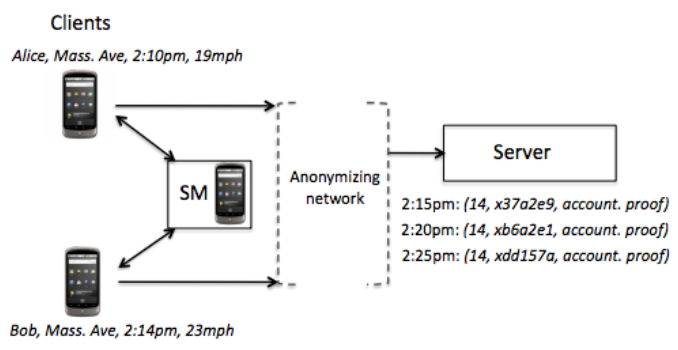
\includegraphics[scale=.7]{C2/privStats}
\caption{Architecture of PrivStats\cite{privstats}}
\end{figure}


\section{Enigma}
Enigma is a theoretical decentralized platform that can perform data computations on an encrypted database \cite{enigma}. It was proposed as a generalized solution for users to put their personal data into use, but with cryptographic guarantees for their privacy.

Its decentralized version has nodes in the system that hold the encrypted data (thus, the user data does leave the phone, but encrypted), and run computations on the data. The interesting part of the proposed solution is the usage of an external blockchain, that acts like a controller of the overall network, managing the access control of each node of the network. In order for the nodes to show a correct and privacy-preserving behaviour, their proofs of correct execution are stored on the blockchain. Since the latter represents a public ledger within the network, any involved entity can check the proofs in order to make sure no user data has been compromised.

Enigma's proposed solution is also worth studying in advance, as it is currently uncertain how the system acts with location data that can reveal meta-information on the user that can, eventually lead to its exposure. This scenario is avoided by PrivStats, by having the SM modules previously described.

\section{Related Work on User Data Markets}
Lately, user data markets are becoming a trending topic among the smartphone users. There are some number of user data markets, such as DataCoup \cite{datacoup}, CitizenMe \cite{citizenme}, people.io \cite{peopleio}, digi.me \cite{digime}.

All of these user data markets, are centralised, collecting all the user data (including location data) to an internal centralised database. Out of the pool of existing user data markets, a concerning number of them are not mentioning anything regarding the privacy or anonymity of the collected data, while the rest of them provide assurances that the collected data is encrypted to some extent, or that is securely stored and not shared with third parties.

The current situation clearly emphasises the need of a decentralised user data market that preserves its users anonymity and privacy.

